\documentclass[12pt]{article}

\usepackage[margin=1.9cm, letterpaper]{geometry}
\usepackage[utf8]{inputenc}
\usepackage{listings}
\usepackage{xcolor}
\usepackage{graphicx}
\usepackage{indentfirst}
\usepackage{tikz}
\usepackage{float}
\usepackage{fancyvrb}
\usepackage{subcaption}
\usepackage{pdfpages}
\usepackage{amsmath}
\usepackage{amssymb}
\usepackage{siunitx}

\usepackage{subfiles}

\usepackage{parskip}
\setlength{\parskip}{1em}
\setlength{\parindent}{2em}

\usetikzlibrary{shapes.geometric, arrows}

\renewcommand{\thesection}{}
\renewcommand{\thesubsection}{}

\lstdefinestyle{mystyle}{
    basicstyle=\ttfamily\footnotesize,
    tabsize=2
}

\tikzstyle{every node}=[font=\scriptsize]

\tikzstyle{terminal} = [rectangle, rounded corners, minimum width=2cm, minimum height=1cm,text centered, draw=black, text width=4.5em]
\tikzstyle{process} = [rectangle, text badly centered, minimum width=3cm, draw=black, text width=5em, node distance=3.5cm]
\tikzstyle{decision} = [diamond,aspect=2, minimum width=1cm,text badly centered, draw=black, text width=6em, node distance=2cm]
\tikzstyle{io} = [trapezium, trapezium left angle=70, trapezium right angle=110, text centered, draw=black, text width=5em]
\tikzstyle{arrow} = [thick,->,>=stealth]

\begin{document}
\begin{titlepage}
    \begin{center}
    \vspace*{1cm}
    
    \textbf{Lab 2}

    \vspace{0.5cm}

    Addressing Modes            
    \vspace{1.5cm}

    \textbf{Hans Jarales (1537516) and Michael Kwok (1548454)}

    \vfill
            
    ECE 212 Lab - Introduction to Microprocessors\\
    Department of Electrical and Computer Engineering\\
    University of Alberta\\
    26 February 2020

   \end{center}
\end{titlepage}

\tableofcontents
\pagebreak

\section{Introduction}
    Address modes refer to the ways in which an operand location can be specified and manipulated. In this lab, data in a specified size is to be stored at adjacent locations in memory. Explored in this lab are different addressing modes used to achieve the purposes of the programs and to take advantage of the structure of the data.
    
    Explored further in tandem with addressing modes are basic arithmetic in ColdFire Assembly. A program is required to perform basic arithmetic (addition, subtraction, multiplication and division) to calculate the area under a curve. To perform multiplication, bitwise operations were used instead which can be done faster than the \Verb#MULU# or \Verb#MULS# instruction for cases when the value is being multiplied or divided by factors of $2^n$.

\section{Design}
\subsection{Part A}
    This part adds two arrays together using different addressing modes, which are Register Indirect with Offset, Indexed Register Indirect and Postincrement Register Indirect. The same array would be used in all 3 addressing modes, and the sum will be saved into another array. Each entry is sized as a longword (32 bits) in all 3 arrays.

    The program calculates the sums of the two arrays by loading one number from memory into a register, adding another from memory into that register then saving the number into it, then copying the number from that register into a memory location. This action is repeated 3 times, using a different memory addressing technique each time.
    
    For Register Indrect with Offset, only the first 3 items in the array are summed. The offsets are manually set in the assembly code. In the program, there is one more copy of the following instructions but with 8 as the offset to access the 3rd longword.

    \begin{verbatim}
    [A2] = Starting address of first array
    [A3] = Starting address of second array
    [A4] = Address to store data at
    
    move.l (a2), d3  /* D3 <- [[A2]] */
    add.l (a3), d3   /* D3 <- D3 + [[A3]] */
    move.l d3, (a4)  /* [A4] <- D3 */
    
    move.l 4(a2), d3 /* D3 <- [4 + [A2]] */
    add.l 4(a3), d3  /* D3 <- D3 + [4 + [A3]] */
    move.l d3, 4(a4) /* [4 + A4] <- D3 */
    \end{verbatim}
    
    \begin{center}
    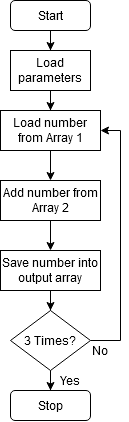
\includegraphics[scale = 0.5]{Lab2/flowchart.png}
    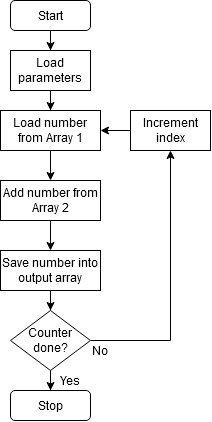
\includegraphics[scale = 0.5]{Lab2/flowchart2.png}
    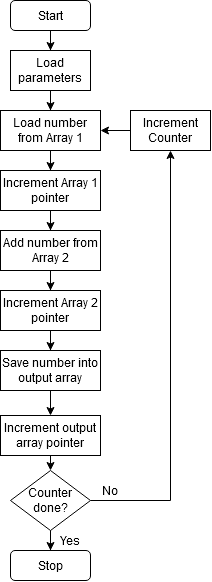
\includegraphics[scale = 0.5]{Lab2/flowchart3.png}
    \end{center}
    
    For Indexed Register Indirect, the entirety of both arrays are added together. The following code fragment will be repeated as the counter gets incremented until it has hit the final index.
    
    \begin{verbatim}
    [A2] = Starting address of first array
    [A3] = Starting address of second array
    [A4] = Address to store data at
    [D7] = Counter for current index
    
    move.l (a2, d7*4), d3 /* D3 <- [[A2 + (D7*4)]] */
    add.l (a3, d7*4), d3  /* D3 <- D3 + [[A3 + (D7*4)]] */
    move.l d3, (a4, d7*4) /* [A4 + (D7*4)] <- D3 */
    \end{verbatim}
    
    For Postincrement Register Indirect, the entirety of both arrays are also added together. Similar to above, the code is repeated for the entire array.
    
    \begin{verbatim}
    [A2] = Starting address of first array
    [A3] = Starting address of second array
    [A4] = Address to store data at
    [D7] = Counter for current index
    
    move.l (a2)+, d3 /* D3 <- [[A2] + 4]; A2 <- A2 + 4 */
    add.l (a3)+, d3  /* D3 <- D3 + [[A3] + 4]; A3 <- A3 + 4 */
    move.l d3, (a4)+ /* [A4] + 4 <- D3; A4 <- A4 + 4  */
    \end{verbatim}

\subsection{Part B}
    This part requires a program to calculate the area under a curve using the \textbf{Trapezoid Rule}
    
    $$A_i = \frac{\Delta x}{2}(y_i + y_{i+1}),~\sum_{i=0}^{N} A_i = \frac{1}{2}\sum_{i=0}^{N}\Delta x(y_i + y_{i+1})$$
        \begin{center}

    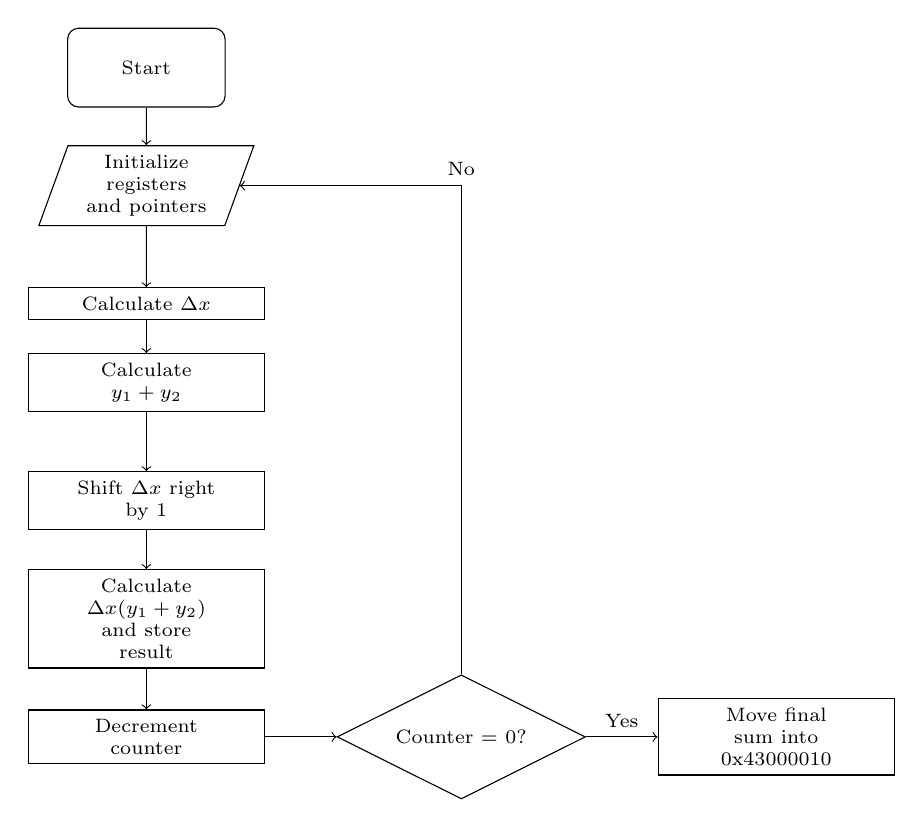
\begin{tikzpicture}[node distance = 1cm]
    
    \node (start) [terminal] {Start};
    \node (initialize) [io, below of = start, yshift = -0.5cm]  {Initialize registers and pointers};
    \node (deltax) [process, below of = initialize, yshift = 2cm] {Calculate $\Delta x$};
    \node (ysum) [process, below of = deltax, yshift = 2.5cm] {Calculate $y_1 + y_2$};
    \node (shift deltax) [process, below of = ysum, yshift = 2cm] {Shift $\Delta x$ right by 1};
    \node (multiplication) [process, below of = shift deltax, yshift = 2cm] {Calculate $\Delta x (y_1 + y_2)$ and store result};
    \node (decrement) [process, below of = multiplication, yshift = 2cm] {Decrement counter};
    \node (depleted counter) [decision, right of = decrement, xshift = 2cm] {Counter = 0?};
    \node (final sum) [process, right of = depleted counter, xshift = 0.5cm] {Move final sum into 0x43000010};
    
    
    \draw[->] (start) -- (initialize);
    \draw[->] (initialize) -- (deltax);
    \draw[->] (deltax) -- (ysum);
    \draw[->] (ysum) -- (shift deltax);
    \draw[->] (shift deltax) -- (multiplication);
    \draw[->] (multiplication) -- (decrement);
    \draw[->] (decrement) -- (depleted counter);
    \draw[->] (depleted counter) |- node[anchor=south]{No} (initialize);
    \draw[->] (depleted counter) -- node[anchor=south]{Yes} (final sum);
    
    
    \end{tikzpicture}
    \end{center}
    The program is required to calculate the final area using the sum of the areas given between ($X_n, Y_n$) and ($X_{n+1}, Y_{n+1}$). These coordinate pairs are located in individual X and Y arrays, with pointers to the beginning of both arrays. A loop is used to perform the area calculations for each pair over the given number of data points. In each loop, the data points $X_n$, $Y_n$, $X_{n+1}$, and $Y_{n+1}$ are moved to individual data registers for calculation using an indirect addressing mode. A single long word post increment is initially applied on the pointers. This in effect calculates the areas from point to point for every loop.
    
    \begin{verbatim}
    Example (1)
    loop:
        move.l (%a2)+, %d3   /* d3 holds initial X points */
        move.l (%a3)+, %d4   /* d4 holds initial Y points */
        move.l (%a2),  %d5   /* d5 holds X endpoint       */
        move.l (%a3),  %d6   /* d6 holds Y endpoint       */
        ...
        calculation
        ...
        Restart Loop until counter reaches 0
    \end{verbatim}
    
   The $\Delta x$ can either be 1, 2, or 4. Rather than writing 3 comparisons for the 3 possibilities of the $\Delta x$, the value is shifted right once. This works because $\Delta x$ is restricted in possibilities. After the shift, $\Delta x$ then becomes $\Delta x' = 0,\,1,\,\text{or }\,2$. The sum $(Y_{n+1} + Y_n)$ is then shifted by $\Delta x'$, in essence being multiplied by 1, 2, or 4. Once the loop is done, a final division by 2 is performed on the resulting sums and the final sum is stored to a designated location. The division by $2$ is moved out of the calculation and left until the end to reduce the amount of rounding errors and improve efficiency by application of the distributive property of division.
    
        \begin{verbatim}
        Example (2)
        [d5] = 2 = 0b10    /* Let dx =  X2 - X1 = 2 */
        [d6] = 3 = 0b11    /* Let Y1 + Y2 = 3       */
        
        asr.l  #1,     %d5   /* Divide d5 content by 2   */
        /* [d5] = 0b1 */
        
        asl.l  %d5,    %d6   /* multiply (Y1 + Y2) by dx */
        /* [d6] = 0b11 is shifted left by 0b1, [d6] now has 0b110 = 6*/
        \end{verbatim}

\section{Testing}
\subsection{Part A}

The program in Part A is simply summing two arrays consecutively. This sum will then be stored into a new array, and each part stores to a different one.

During the lab, it was tested with different datasets, correctly obtaining the sums each time. Below is a screenshot of the result from the test program for DataStorage.s:

\begin{center}
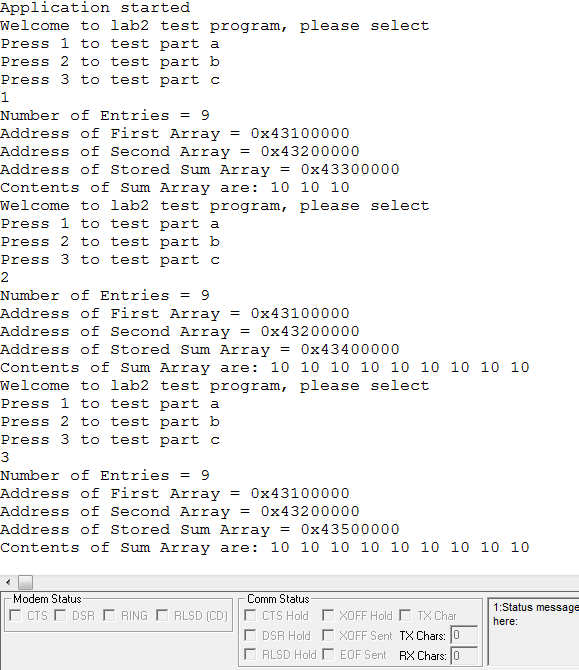
\includegraphics[scale = 0.5]{./Lab2a.PNG}
\end{center}

\subsection{Part B}
The Part B program in summary should accumulate a sum obtained from the calculated areas given from a set of consecutive x and y coordinate pairs on a curve. This accumulated sum should be the returned, final answer.

The Part B program was tested against different data point scenarios, successfully and consistently obtaining the correct areas. Below is an example calculation using DataStorage5.s:

\begin{center}
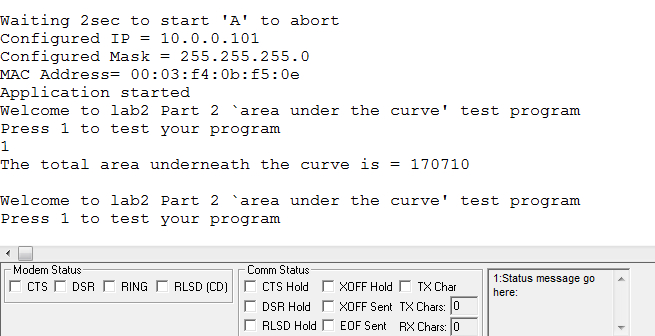
\includegraphics[scale = 0.5]{Lab2/Lab2b.jpg}
\end{center}

\section{Questions}
 \begin{enumerate}
     \item \begin{itemize}
         \item For programs where the address offsets are known, Register Indirect allows you to access multiple addresses without modifying a register without a loop.
         \item For address accesses where the scaling might not be the same as instruction access size, Indexed Register Indirect allows you to set the scaling factor and also does not modify the address register being used.
         \item For sequential reads, Postincrement Register Indirect is easier and does not require a data register ot use as an index.
     \end{itemize}
     
     \item The MULU (unsigned multiplication) instruction can be used in place of comparisons (CMP) and conditional branching that would otherwise need to be implemented in the situation that $ \Delta x$ is not restricted to the values 1,2 and 4. The operation $\Delta x * (y_1 + y_2)$ can take place by performing a MULU instruction between the locations holding these values.
     
     \item The function was defined as $f(x) = x^2$. Since we used DataStorage5.s, we know that the domain of x is $[0, 80]$, so the calculation done was $\int_{0}^{80} x^2 dx = \num{170666.6}$. This number is smaller than our obtained value of \num{170710}, with an error of \num[round-mode = figures, round-precision=2]{0.02542969743}\%
\end{enumerate}

\section{Conclusions}
    Making use of addressing modes wherever possible creates shorter and easier to read code.  In this lab, the data gathered for analysis were stored in arrays. In this, address pointer increments can then be conveniently utilized to gather consecutive data points when performing the same calculation multiple times by utilizing a loop.
    
    Manually manipulating the address values proves a more tedious task. Doing so results in more lines of code to be read, and an increase in risk of possible errors in instructions and calculations.
    
    For further efficiency, alternatives to conditional branching should be considered and explored. In Part B, a solution was implemented to reduce potentially several lines of code to a single instruction. With a consistently correct result, the program proved more efficient and effective than the more intuitive approach.
    
\pagebreak

\section{Appendix}
\renewcommand{\thepage}{}
\subsection{Part A Assembler Code}
\lstinputlisting[language={[Motorola68k]Assembler}, style={mystyle}]{Lab2a.s}
\pagebreak
\subsection{Part B Assembler Code}
\lstinputlisting[language={[Motorola68k]Assembler}, style={mystyle}]{Lab2b.s}

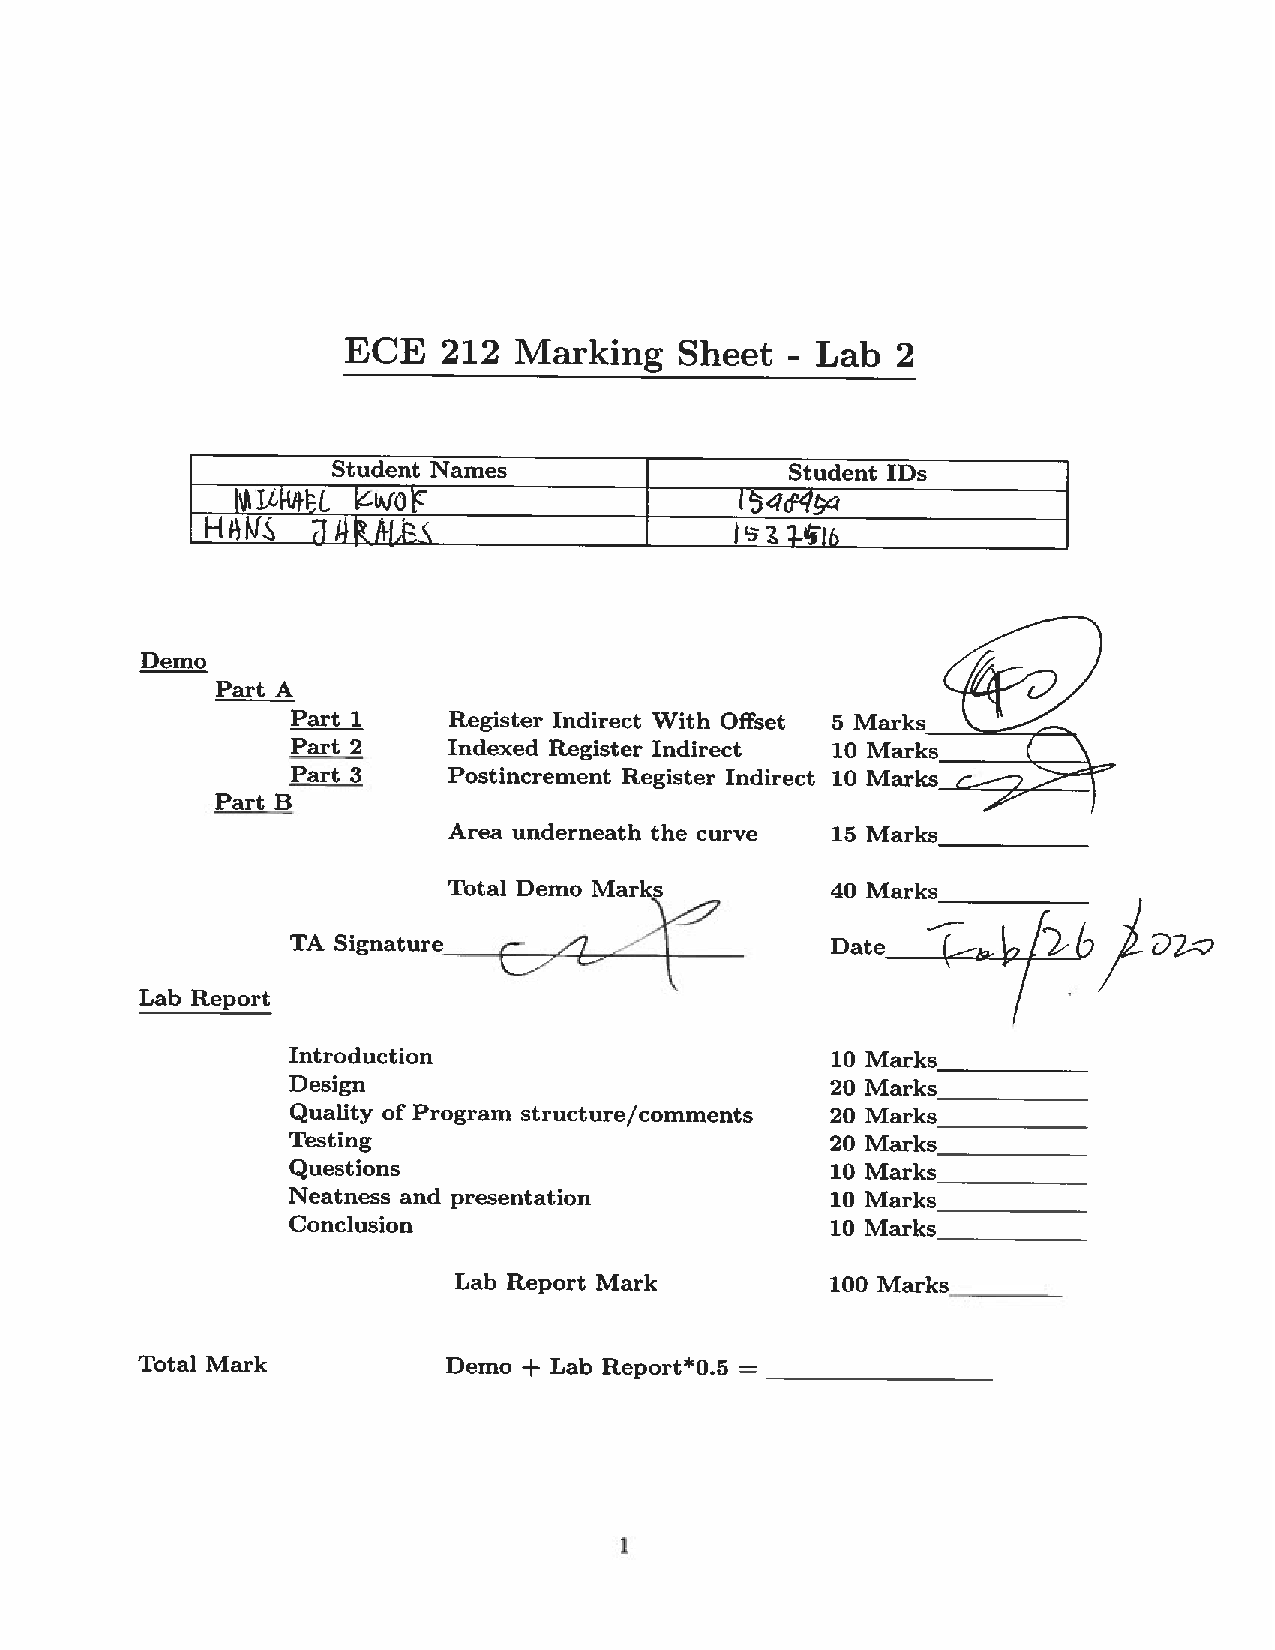
\includepdf[pages=-]{Lab2MarkingSheet.pdf}

\end{document}